%% Created by Maple 17.00, Linux
%% Source Worksheet: Uncertain.mw
%% Generated: Thu Jan 14 18:47:09 BRT 2021
\documentclass{article}
\usepackage{maplestd2e}
\def\emptyline{\vspace{12pt}}
\begin{document}
\pagestyle{empty}
\DefineParaStyle{Maple Heading 1}
\DefineParaStyle{Maple Text Output}
\DefineParaStyle{Maple Dash Item}
\DefineParaStyle{Maple Bullet Item}
\DefineParaStyle{Maple Normal}
\DefineParaStyle{Maple Heading 4}
\DefineParaStyle{Maple Heading 3}
\DefineParaStyle{Maple Heading 2}
\DefineParaStyle{Maple Warning}
\DefineParaStyle{Maple Title}
\DefineParaStyle{Maple Error}
\DefineCharStyle{Maple Hyperlink}
\DefineCharStyle{Maple 2D Math}
\DefineCharStyle{Maple Maple Input}
\DefineCharStyle{Maple 2D Output}
\DefineCharStyle{Maple 2D Input}
\mapleinline{inert}{2d}{restart; -1}{\[\displaystyle \]}
\begin{Maple Normal}{
\begin{Maple Normal}{
Obs 1: Pelo avaliado, o circuito equivalente na amostragem entrada no modo diferencial e terminação única são iguais. A incerteza dos dois acabam dependendo exclusivamente da fonte e0 e tambem são iguais. Ppara facilitar, RsCs é considerado uma só variável, as incertezas referente a estes valores já foram previamente calculadas por meio da regra da soma(entre resistores) e produto(entre capacitores). Todas as incertezas são absolutas.}\end{Maple Normal}

\begin{Maple Normal}{
Obs 1: Pelo avaliado, o circuito equivalente na amostragem entrada no modo diferencial e terminação única são iguais. A incerteza dos dois acabam dependendo exclusivamente da fonte e0 e tambem são iguais. Ppara facilitar, RsCs é considerado uma só variável, as incertezas referente a estes valores já foram previamente calculadas por meio da regra da soma(entre resistores) e produto(entre capacitores). Todas as incertezas são absolutas.\mapleinline{inert}{2d}{}{$\displaystyle $}
}\end{Maple Normal}

}\end{Maple Normal}

\begin{Maple Normal}{
\begin{Maple Normal}{
}\end{Maple Normal}
}\end{Maple Normal}
\begin{Maple Normal}{
\begin{Maple Normal}{
1 - Calculo da incerteza para a etapa de amostragem de entrada, considerando e0 livre de incertezas (referente ao arquivo uncert\_input\_samplig.m)}\end{Maple Normal}

}\end{Maple Normal}

\begin{Maple Normal}{
\begin{Maple Normal}{
}\end{Maple Normal}
}\end{Maple Normal}
\mapleinline{inert}{2d}{Vcs := e0*(1-exp(-t/RsCs))}{\[\displaystyle {\it Vcs}\, := \,{\it e0}\, \left( 1-{{\rm e}^{-{\frac {t}{{\it RsCs}}}}} \right) \]}
\begin{maplegroup}
\mapleresult
\begin{maplelatex}
\mapleinline{inert}{2d}{e0*(1-exp(-t/RsCs))}{\[\displaystyle {\it e0}\, \left( 1-{{\rm e}^{-{\frac {t}{{\it RsCs}}}}} \right) \]}
\end{maplelatex}
\end{maplegroup}
\begin{Maple Normal}{
\begin{Maple Normal}{
\mapleinline{inert}{2d}{}{\[\displaystyle \]}
}\end{Maple Normal}
}\end{Maple Normal}
\begin{Maple Normal}{
\begin{Maple Normal}{
Incerteza de Vcs, considerando apenas Rs e Cs como fontes de incerteza é dada por:}\end{Maple Normal}

}\end{Maple Normal}

\begin{Maple Normal}{
\begin{Maple Normal}{
}\end{Maple Normal}
}\end{Maple Normal}
\mapleinline{inert}{2d}{sigma[Vcs] := abs(diff(Vcs, RsCs))*sigma[RsCs]}{\[\displaystyle \sigma_{{{\it Vcs}}}\, := \, \left| {\frac {d}{d{\it RsCs}}}{\it Vcs} \right| \sigma_{{{\it RsCs}}}\]}
\begin{maplegroup}
\mapleresult
\begin{maplelatex}
\mapleinline{inert}{2d}{exp(-Re(t/RsCs))*abs(e0*t/RsCs^2)*sigma[RsCs]}{\[\displaystyle {{\rm e}^{-{\it Re} \left( {\frac {t}{{\it RsCs}}} \right) }} \left| {\frac {{\it e0}\,t}{{{\it RsCs}}^{2}}} \right| \sigma_{{{\it RsCs}}}\]}
\end{maplelatex}
\end{maplegroup}
\begin{Maple Normal}{
\begin{Maple Normal}{
\mapleinline{inert}{2d}{}{\[\displaystyle \]}
}\end{Maple Normal}
}\end{Maple Normal}
\begin{center}
\begin{Maple Normal}{
\begin{center}
\begin{Maple Normal}{
\raisebox{4.819444444444445in}{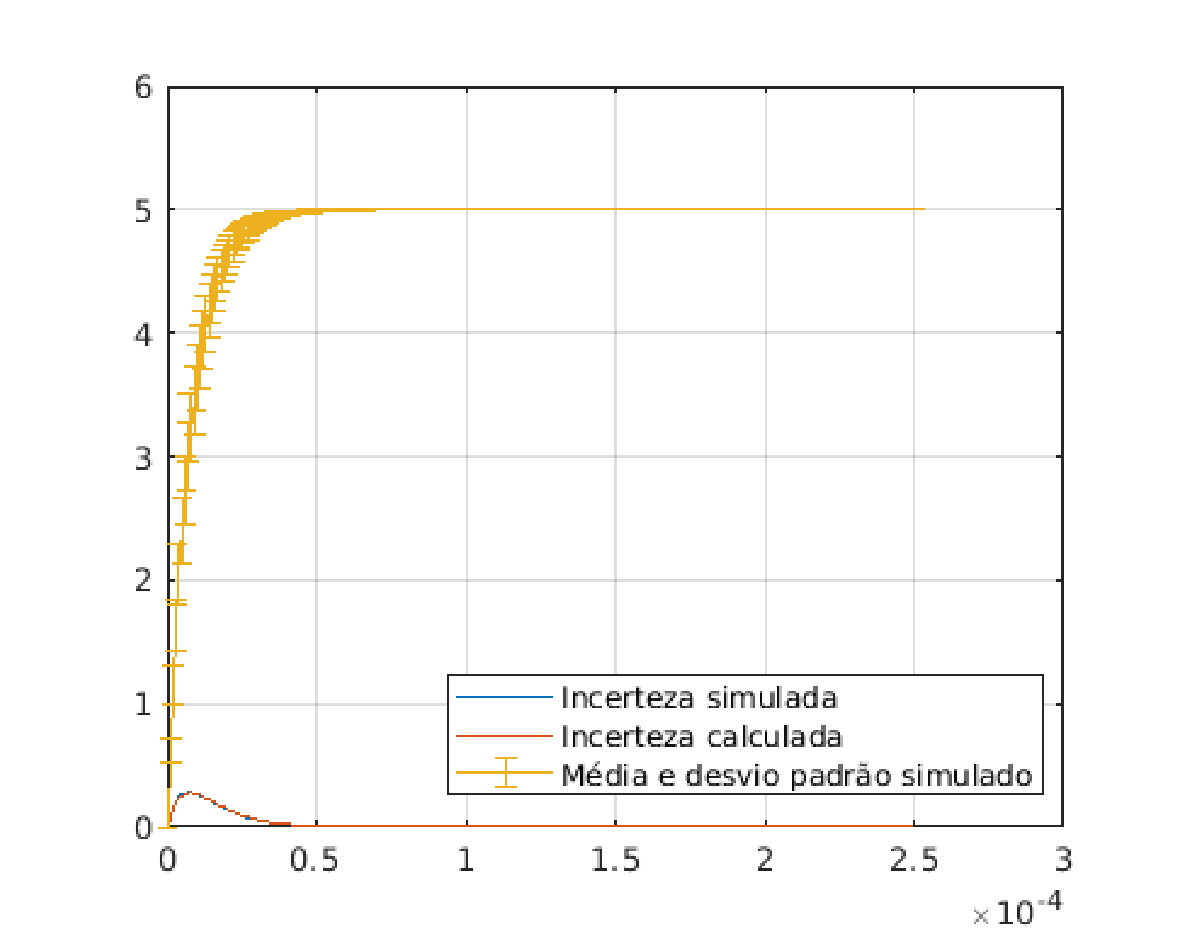
\includegraphics[keepaspectratio,totalheight=5.638888888888889in,angle=-90]{Uncertainimage0.eps}}\mapleinline{inert}{2d}{}{$\displaystyle $}
}\end{Maple Normal}
\end{center}
}\end{Maple Normal}
\end{center}
\begin{center}
\begin{Maple Normal}{
\begin{center}
\begin{Maple Normal}{
}\end{Maple Normal}
\end{center}
}\end{Maple Normal}
\end{center}
\begin{Maple Normal}{
\begin{Maple Normal}{
\mapleinline{inert}{2d}{}{\[\displaystyle \]}
}\end{Maple Normal}
}\end{Maple Normal}
\begin{Maple Normal}{
\begin{Maple Normal}{
\mapleinline{inert}{2d}{}{\[\displaystyle \]}
}\end{Maple Normal}
}\end{Maple Normal}
\mapleinline{inert}{2d}{restart; -1}{\[\displaystyle \]}
\begin{Maple Normal}{
\begin{Maple Normal}{
2 -Calculo da incerteza para a etapa de amplificação, considerando Vcs livre de incertezas (referente ao arquivo uncert\_amplification.m)}\end{Maple Normal}

}\end{Maple Normal}

\begin{Maple Normal}{
\begin{Maple Normal}{
\mapleinline{inert}{2d}{}{\[\displaystyle \]}
}\end{Maple Normal}
}\end{Maple Normal}
\mapleinline{inert}{2d}{Va := Vcs*(1+t/RaCa)}{\[\displaystyle {\it Va}\, := \,{\it Vcs}\, \left( 1+{\frac {t}{{\it RaCa}}} \right) \]}
\begin{maplegroup}
\mapleresult
\begin{maplelatex}
\mapleinline{inert}{2d}{Vcs*(1+t/RaCa)}{\[\displaystyle {\it Vcs}\, \left( 1+{\frac {t}{{\it RaCa}}} \right) \]}
\end{maplelatex}
\end{maplegroup}
\begin{Maple Normal}{
\begin{Maple Normal}{
\mapleinline{inert}{2d}{}{\[\displaystyle \]}
}\end{Maple Normal}
}\end{Maple Normal}
\begin{Maple Normal}{
\begin{Maple Normal}{
Incerteza de Va, considerando apenas Ra e Ca como fontes de incerteza é dada por:}\end{Maple Normal}

}\end{Maple Normal}

\mapleinline{inert}{2d}{sigma[Va] := abs(diff(Va, RaCa))*sigma[RaCa]}{\[\displaystyle \sigma_{{{\it Va}}}\, := \, \left| {\frac {d}{d{\it RaCa}}}{\it Va} \right| \sigma_{{{\it RaCa}}}\]}
\begin{maplegroup}
\mapleresult
\begin{maplelatex}
\mapleinline{inert}{2d}{abs(Vcs*t/RaCa^2)*sigma[RaCa]}{\[\displaystyle  \left| {\frac {{\it Vcs}\,t}{{{\it RaCa}}^{2}}} \right| \sigma_{{{\it RaCa}}}\]}
\end{maplelatex}
\end{maplegroup}
\begin{Maple Normal}{
\begin{Maple Normal}{
\mapleinline{inert}{2d}{}{\[\displaystyle \]}
}\end{Maple Normal}
}\end{Maple Normal}
\begin{center}
\begin{Maple Normal}{
\begin{center}
\begin{Maple Normal}{
\raisebox{5.986111111111111in}{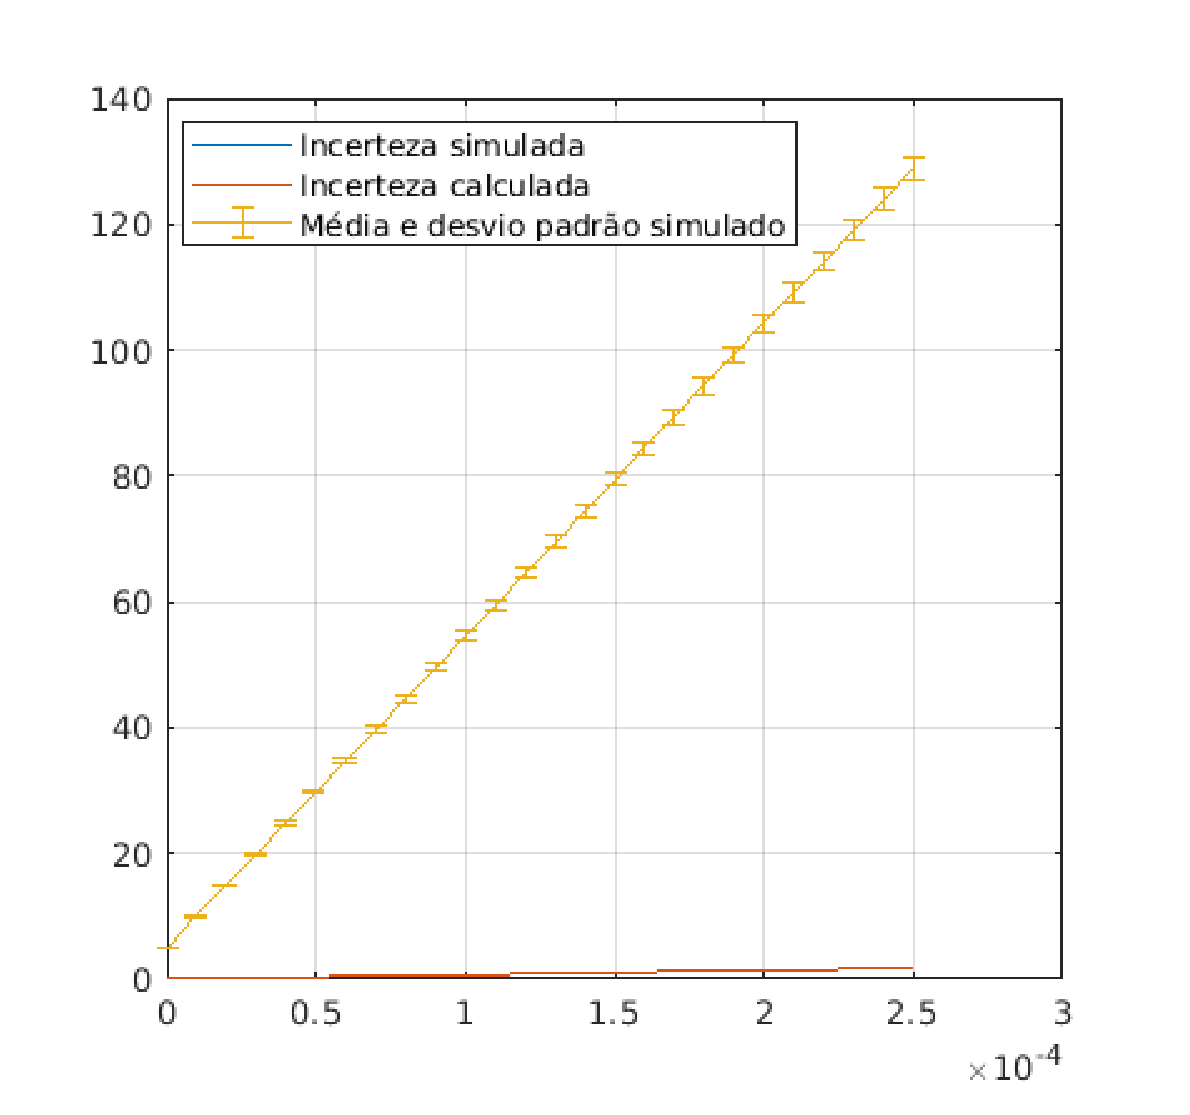
\includegraphics[keepaspectratio,totalheight=6.416666666666667in,angle=-90]{Uncertainimage1.eps}}}\end{Maple Normal}
\end{center}
}\end{Maple Normal}
\end{center}
\mapleinline{inert}{2d}{restart; -1}{\[\displaystyle \]}
\begin{Maple Normal}{
\begin{Maple Normal}{
3 -Calculo da incerteza para a etapa de amostragem de saída, considerando Va livre de incertezas (referente ao arquivo uncert\_output\_samplig.m)}\end{Maple Normal}

}\end{Maple Normal}

\begin{Maple Normal}{
\begin{Maple Normal}{
\mapleinline{inert}{2d}{}{\[\displaystyle \]}
}\end{Maple Normal}
}\end{Maple Normal}
\mapleinline{inert}{2d}{Vo := Va*(1-exp(-t/RoCo))}{\[\displaystyle {\it Vo}\, := \,{\it Va}\, \left( 1-{{\rm e}^{-{\frac {t}{{\it RoCo}}}}} \right) \]}
\begin{maplegroup}
\mapleresult
\begin{maplelatex}
\mapleinline{inert}{2d}{Va*(1-exp(-t/RoCo))}{\[\displaystyle {\it Va}\, \left( 1-{{\rm e}^{-{\frac {t}{{\it RoCo}}}}} \right) \]}
\end{maplelatex}
\end{maplegroup}
\begin{Maple Normal}{
\begin{Maple Normal}{
\mapleinline{inert}{2d}{}{\[\displaystyle \]}
}\end{Maple Normal}
}\end{Maple Normal}
\begin{Maple Normal}{
\begin{Maple Normal}{
Incerteza de Vo, considerando apenas Ro e Co como fontes de incerteza é dada por:}\end{Maple Normal}

}\end{Maple Normal}

\mapleinline{inert}{2d}{sigma[Vo] := abs(diff(Vo, RoCo))*sigma[RoCo]}{\[\displaystyle \sigma_{{{\it Vo}}}\, := \, \left| {\frac {d}{d{\it RoCo}}}{\it Vo} \right| \sigma_{{{\it RoCo}}}\]}
\begin{maplegroup}
\mapleresult
\begin{maplelatex}
\mapleinline{inert}{2d}{exp(-Re(t/RoCo))*abs(Va*t/RoCo^2)*sigma[RoCo]}{\[\displaystyle {{\rm e}^{-{\it Re} \left( {\frac {t}{{\it RoCo}}} \right) }} \left| {\frac {{\it Va}\,t}{{{\it RoCo}}^{2}}} \right| \sigma_{{{\it RoCo}}}\]}
\end{maplelatex}
\end{maplegroup}
\begin{Maple Normal}{
\begin{Maple Normal}{
\mapleinline{inert}{2d}{}{\[\displaystyle \]}
}\end{Maple Normal}
}\end{Maple Normal}
\begin{center}
\begin{Maple Normal}{
\begin{center}
\begin{Maple Normal}{
\raisebox{5.430555555555555in}{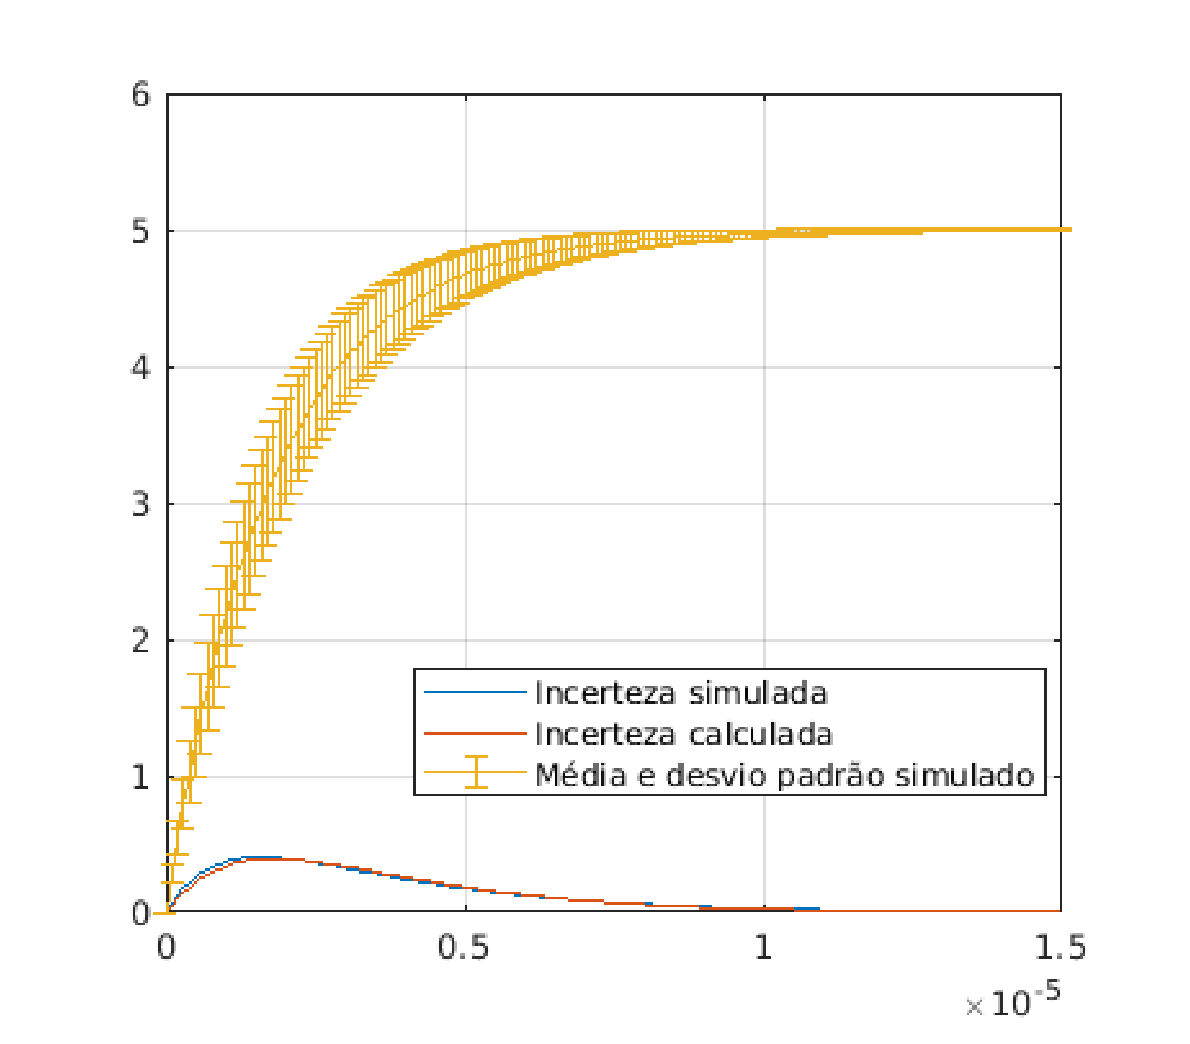
\includegraphics[keepaspectratio,totalheight=6.236111111111111in,angle=-90]{Uncertainimage2.eps}}}\end{Maple Normal}
\end{center}
}\end{Maple Normal}
\end{center}
\begin{center}
\begin{Maple Normal}{
\begin{center}
\begin{Maple Normal}{
}\end{Maple Normal}
\end{center}
}\end{Maple Normal}
\end{center}
\begin{center}
\begin{Maple Normal}{
\begin{center}
\begin{Maple Normal}{
}\end{Maple Normal}
\end{center}
}\end{Maple Normal}
\end{center}
\begin{center}
\begin{Maple Normal}{
\begin{center}
\begin{Maple Normal}{
}\end{Maple Normal}
\end{center}
}\end{Maple Normal}
\end{center}
\begin{center}
\begin{Maple Normal}{
\begin{center}
\begin{Maple Normal}{
}\end{Maple Normal}
\end{center}
}\end{Maple Normal}
\end{center}
\begin{center}
\begin{Maple Normal}{
\begin{center}
\begin{Maple Normal}{
}\end{Maple Normal}
\end{center}
}\end{Maple Normal}
\end{center}
\mapleinline{inert}{2d}{restart; -1}{\[\displaystyle \]}
\begin{Maple Normal}{
\begin{Maple Normal}{
4 -Calculo da incerteza para a etapa de amostragem de saída, considerando e0 fonte de incertezas (referente ao arquivo uncert\_source\_plus\_input.m)}\end{Maple Normal}

}\end{Maple Normal}

\begin{Maple Normal}{
\begin{Maple Normal}{
\mapleinline{inert}{2d}{}{\[\displaystyle \]}
}\end{Maple Normal}
}\end{Maple Normal}
\mapleinline{inert}{2d}{Vcs := e0*(1-exp(-t/RsCs))}{\[\displaystyle {\it Vcs}\, := \,{\it e0}\, \left( 1-{{\rm e}^{-{\frac {t}{{\it RsCs}}}}} \right) \]}
\begin{maplegroup}
\mapleresult
\begin{maplelatex}
\mapleinline{inert}{2d}{e0*(1-exp(-t/RsCs))}{\[\displaystyle {\it e0}\, \left( 1-{{\rm e}^{-{\frac {t}{{\it RsCs}}}}} \right) \]}
\end{maplelatex}
\end{maplegroup}
\mapleinline{inert}{2d}{sigma[Vcs] := sqrt((sigma[e0]*(diff(Vcs, e0)))^2+(sigma[RsCs]*(diff(Vcs, RsCs)))^2)}{\[\displaystyle \sigma_{{{\it Vcs}}}\, := \, \sqrt{{\sigma_{{{\it e0}}}}^{2} \left( {\frac {d}{d{\it e0}}}{\it Vcs} \right) ^{2}+{\sigma_{{{\it RsCs}}}}^{2} \left( {\frac {d}{d{\it RsCs}}}{\it Vcs} \right) ^{2}\\
\mbox{}}\]}
\begin{maplegroup}
\mapleresult
\begin{maplelatex}
\mapleinline{inert}{2d}{sqrt(sigma[e0]^2*(1-exp(-t/RsCs))^2+sigma[RsCs]^2*e0^2*t^2*(exp(-t/RsCs))^2/RsCs^4)}{\[\displaystyle  \sqrt{{\sigma_{{{\it e0}}}}^{2} \left( 1-{{\rm e}^{-{\frac {t}{{\it RsCs}}}}} \right) ^{2}+{\sigma_{{{\it RsCs}}}}^{2}{{\it e0}}^{2}{t}^{2} \left( {{\rm e}^{-{\frac {t}{{\it RsCs}}}}} \right) ^{2}{{\it RsCs}}^{-4}\\
\mbox{}}\]}
\end{maplelatex}
\end{maplegroup}
\begin{Maple Normal}{
\begin{Maple Normal}{
\mapleinline{inert}{2d}{}{\[\displaystyle \]}
}\end{Maple Normal}
}\end{Maple Normal}
\begin{center}
\begin{Maple Normal}{
\begin{center}
\begin{Maple Normal}{
\raisebox{5.083333333333333in}{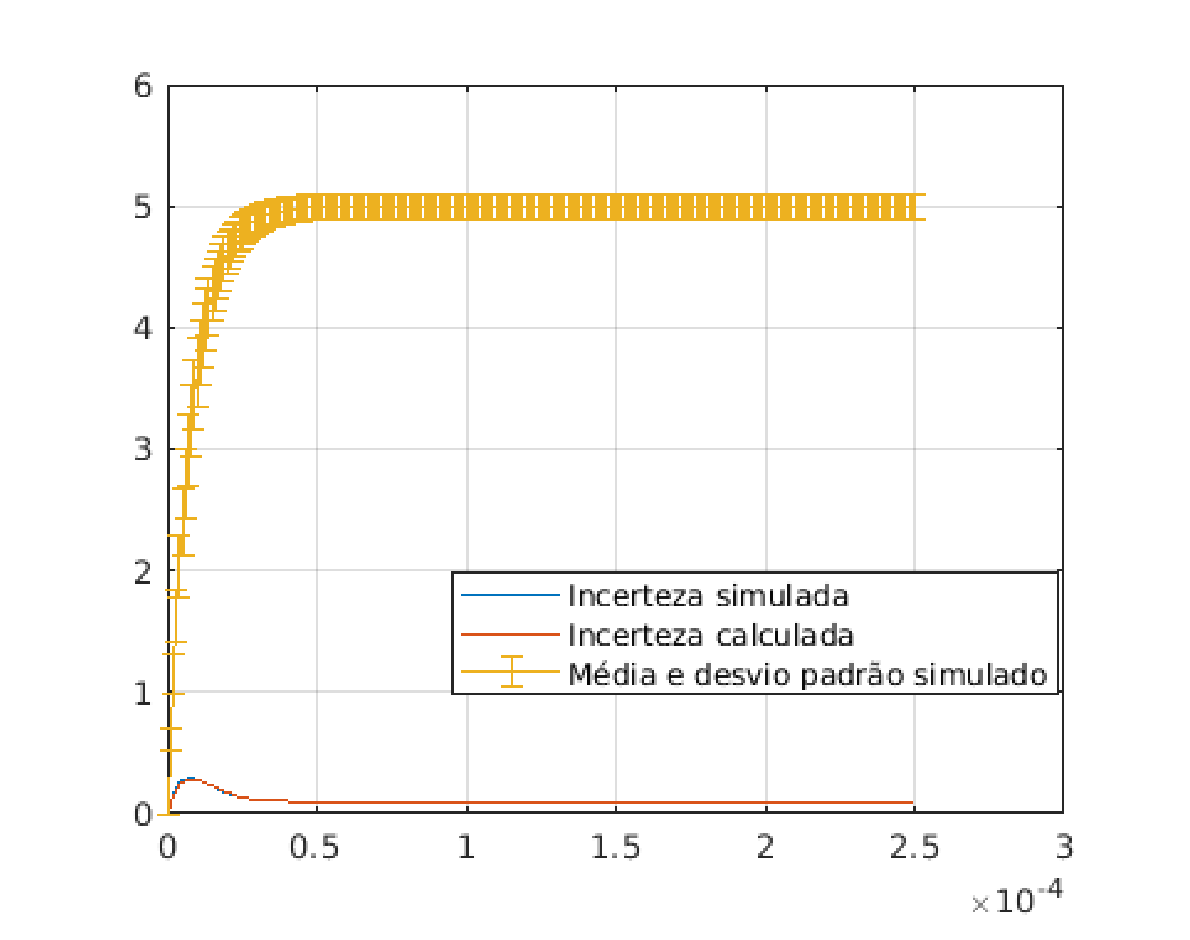
\includegraphics[keepaspectratio,totalheight=6.5in,angle=-90]{Uncertainimage3.eps}}}\end{Maple Normal}
\end{center}
}\end{Maple Normal}
\end{center}
\begin{center}
\begin{Maple Normal}{
\begin{center}
\begin{Maple Normal}{
}\end{Maple Normal}
\end{center}
}\end{Maple Normal}
\end{center}
\begin{center}
\begin{Maple Normal}{
\begin{center}
\begin{Maple Normal}{
}\end{Maple Normal}
\end{center}
}\end{Maple Normal}
\end{center}
\begin{center}
\begin{Maple Normal}{
\begin{center}
\begin{Maple Normal}{
}\end{Maple Normal}
\end{center}
}\end{Maple Normal}
\end{center}
\begin{center}
\begin{Maple Normal}{
\begin{center}
\begin{Maple Normal}{
}\end{Maple Normal}
\end{center}
}\end{Maple Normal}
\end{center}
\begin{center}
\begin{Maple Normal}{
\begin{center}
\begin{Maple Normal}{
}\end{Maple Normal}
\end{center}
}\end{Maple Normal}
\end{center}
\begin{Maple Normal}{
\begin{Maple Normal}{
\mapleinline{inert}{2d}{}{\[\displaystyle \]}
}\end{Maple Normal}
}\end{Maple Normal}
\mapleinline{inert}{2d}{restart; -1}{\[\displaystyle \]}
\begin{Maple Normal}{
\begin{Maple Normal}{
5 - Calculo da incerteza para todas as etapas do PGA, considerando e0 fonte de incertezas (referente ao arquivo uncert\_PGA.m)}\end{Maple Normal}

}\end{Maple Normal}

\begin{Maple Normal}{
\begin{Maple Normal}{
São desconsiderados aspectos reais do funcionamento do circuito. Etapa feita apenas para comparação posterior.}\end{Maple Normal}

}\end{Maple Normal}

\begin{Maple Normal}{
\begin{Maple Normal}{
}\end{Maple Normal}
}\end{Maple Normal}
\begin{Maple Normal}{
\begin{Maple Normal}{
}\end{Maple Normal}
}\end{Maple Normal}
\mapleinline{inert}{2d}{Vcs := e0*(1-exp(-t/RsCs))}{\[\displaystyle {\it Vcs}\, := \,{\it e0}\, \left( 1-{{\rm e}^{-{\frac {t}{{\it RsCs}}}}} \right) \]}
\begin{maplegroup}
\mapleresult
\begin{maplelatex}
\mapleinline{inert}{2d}{e0*(1-exp(-t/RsCs))}{\[\displaystyle {\it e0}\, \left( 1-{{\rm e}^{-{\frac {t}{{\it RsCs}}}}} \right) \]}
\end{maplelatex}
\end{maplegroup}
\mapleinline{inert}{2d}{Ga := 1+t/RaCa}{\[\displaystyle {\it Ga}\, := \,1+{\frac {t}{{\it RaCa}}}\]}
\begin{maplegroup}
\mapleresult
\begin{maplelatex}
\mapleinline{inert}{2d}{1+t/RaCa}{\[\displaystyle 1+{\frac {t}{{\it RaCa}}}\]}
\end{maplelatex}
\end{maplegroup}
\mapleinline{inert}{2d}{Va := Vcs*Ga}{\[\displaystyle {\it Va}\, := \,{\it Vcs}\,{\it Ga}\]}
\begin{maplegroup}
\mapleresult
\begin{maplelatex}
\mapleinline{inert}{2d}{e0*(1-exp(-t/RsCs))*(1+t/RaCa)}{\[\displaystyle {\it e0}\, \left( 1-{{\rm e}^{-{\frac {t}{{\it RsCs}}}}} \right)  \left( 1+{\frac {t}{{\it RaCa}}} \right) \]}
\end{maplelatex}
\end{maplegroup}
\mapleinline{inert}{2d}{Vo := 1-exp(-t/RoCo)}{\[\displaystyle {\it Vo}\, := \,1-{{\rm e}^{-{\frac {t}{{\it RoCo}}}}}\]}
\begin{maplegroup}
\mapleresult
\begin{maplelatex}
\mapleinline{inert}{2d}{1-exp(-t/RoCo)}{\[\displaystyle 1-{{\rm e}^{-{\frac {t}{{\it RoCo}}}}}\]}
\end{maplelatex}
\end{maplegroup}
\mapleinline{inert}{2d}{Vf := Va*Vo}{\[\displaystyle {\it Vf}\, := \,{\it Va}\,{\it Vo}\]}
\begin{maplegroup}
\mapleresult
\begin{maplelatex}
\mapleinline{inert}{2d}{e0*(1-exp(-t/RsCs))*(1+t/RaCa)*(1-exp(-t/RoCo))}{\[\displaystyle {\it e0}\, \left( 1-{{\rm e}^{-{\frac {t}{{\it RsCs}}}}} \right)  \left( 1+{\frac {t}{{\it RaCa}}} \right)  \left( 1-{{\rm e}^{-{\frac {t}{{\it RoCo}}}}} \right) \]}
\end{maplelatex}
\end{maplegroup}
\begin{Maple Normal}{
\begin{Maple Normal}{
\mapleinline{inert}{2d}{}{\[\displaystyle \]}
}\end{Maple Normal}
}\end{Maple Normal}
\mapleinline{inert}{2d}{sigma[Vf] := sqrt((sigma[e0]*(diff(Vf, e0)))^2+(sigma[RsCs]*(diff(Vf, RsCs)))^2+(sigma[RaCa]*(diff(Vf, RaCa)))^2+(sigma[RoCo]*(diff(Vf, RoCo)))^2)}{\[\displaystyle \sigma_{{{\it Vf}}}\, := \, \sqrt{{\sigma_{{{\it e0}}}}^{2} \left( {\frac {d}{d{\it e0}}}{\it Vf} \right) ^{2}+{\sigma_{{{\it RsCs}}}}^{2} \left( {\frac {d}{d{\it RsCs}}}{\it Vf} \right) ^{2}\\
\mbox{}+{\sigma_{{{\it RaCa}}}}^{2} \left( {\frac {d}{d{\it RaCa}}}{\it Vf} \right) ^{2}+{\sigma_{{{\it RoCo}}}}^{2} \left( {\frac {d}{d{\it RoCo}}}{\it Vf} \right) ^{2}}\]}
\begin{maplegroup}
\mapleresult
\begin{maplelatex}
\mapleinline{inert}{2d}{sqrt(sigma[e0]^2*(1-exp(-t/RsCs))^2*(1+t/RaCa)^2*(1-exp(-t/RoCo))^2+sigma[RsCs]^2*e0^2*t^2*(exp(-t/RsCs))^2*(1+t/RaCa)^2*(1-exp(-t/RoCo))^2/RsCs^4+sigma[RaCa]^2*e0^2*(1-exp(-t/RsCs))^2*t^2*(1-exp(-t/RoCo))^2/RaCa^4+sigma[RoCo]^2*e0^2*(1-exp(-t/RsCs))^2*(1+t/RaCa)^2*t^2*(exp(-t/RoCo))^2/RoCo^4)}{\[\displaystyle  \sqrt{{\sigma_{{{\it e0}}}}^{2} \left( 1-{{\rm e}^{-{\frac {t}{{\it RsCs}}}}} \right) ^{2} \left( 1+{\frac {t}{{\it RaCa}}} \right) ^{2}\\
\mbox{} \left( 1-{{\rm e}^{-{\frac {t}{{\it RoCo}}}}} \right) ^{2}+{\sigma_{{{\it RsCs}}}}^{2}{{\it e0}}^{2}{t}^{2} \left( {{\rm e}^{-{\frac {t}{{\it RsCs}}}}} \right) ^{2} \left( 1+{\frac {t}{{\it RaCa}}} \right) ^{2} \left( 1-{{\rm e}^{-{\frac {t}{{\it RoCo}}}}} \right) ^{2}{{\it RsCs}}^{-4}\\
\mbox{}+{\sigma_{{{\it RaCa}}}}^{2}{{\it e0}}^{2} \left( 1-{{\rm e}^{-{\frac {t}{{\it RsCs}}}}} \right) ^{2}{t}^{2} \left( 1-{{\rm e}^{-{\frac {t}{{\it RoCo}}}}} \right) ^{2}{{\it RaCa}}^{-4}+{\sigma_{{{\it RoCo}}}}^{2}{{\it e0}}^{2} \left( 1-{{\rm e}^{-{\frac {t}{{\it RsCs}}}}} \right) ^{2} \left( 1+{\frac {t}{{\it RaCa}}} \right) ^{2}{t}^{2} \left( {{\rm e}^{-{\frac {t}{{\it RoCo}}}}} \right) ^{2}{{\it RoCo}}^{-4}\\
\mbox{}}\]}
\end{maplelatex}
\end{maplegroup}
\begin{Maple Normal}{
\begin{Maple Normal}{
\mapleinline{inert}{2d}{}{\[\displaystyle \]}
}\end{Maple Normal}
}\end{Maple Normal}
\begin{center}
\begin{Maple Normal}{
\begin{center}
\begin{Maple Normal}{
\raisebox{5.333333333333333in}{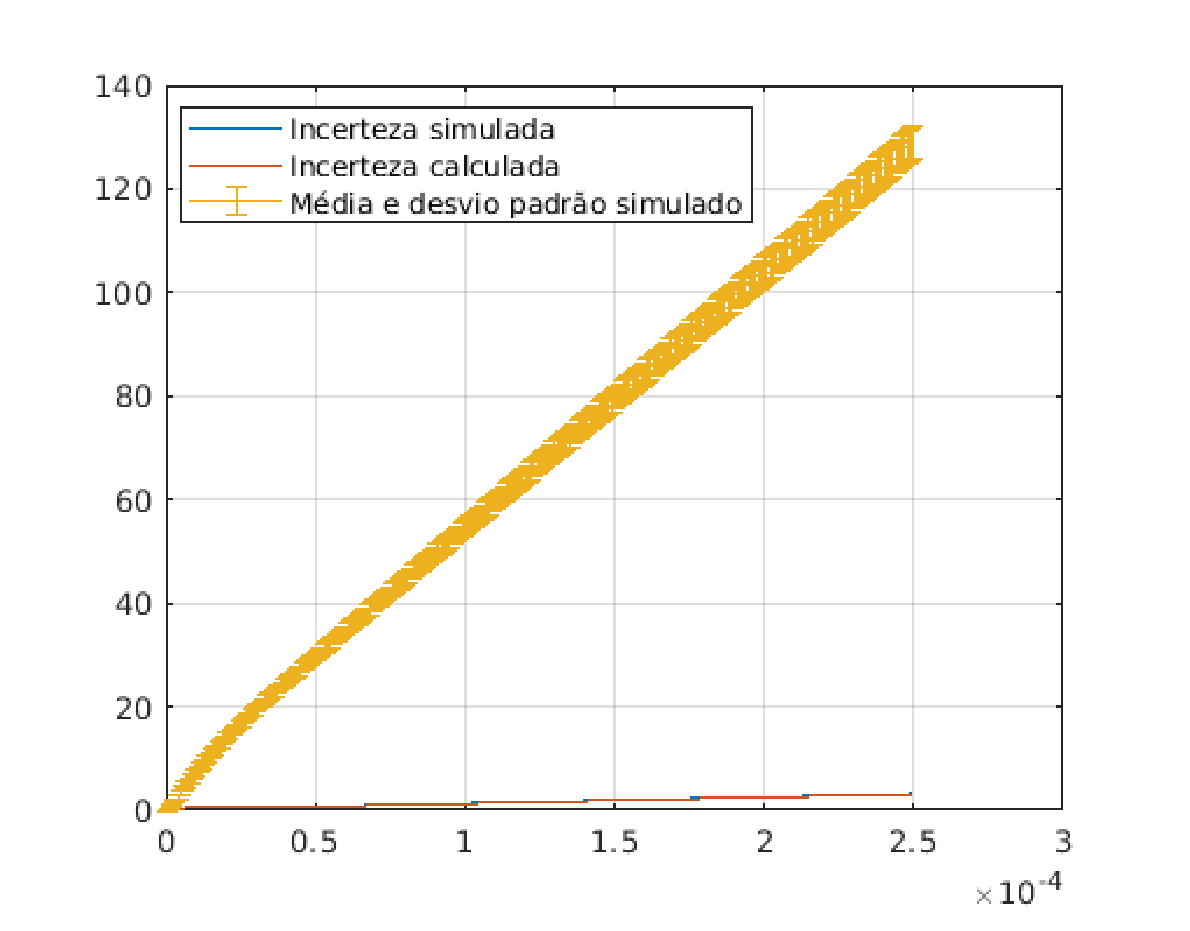
\includegraphics[keepaspectratio,totalheight=6.888888888888889in,angle=-90]{Uncertainimage4.eps}}}\end{Maple Normal}
\end{center}
}\end{Maple Normal}
\end{center}
\begin{center}
\begin{Maple Normal}{
\begin{center}
\begin{Maple Normal}{
}\end{Maple Normal}
\end{center}
}\end{Maple Normal}
\end{center}
\begin{center}
\begin{Maple Normal}{
\begin{center}
\begin{Maple Normal}{
}\end{Maple Normal}
\end{center}
}\end{Maple Normal}
\end{center}
\begin{center}
\begin{Maple Normal}{
\begin{center}
\begin{Maple Normal}{
}\end{Maple Normal}
\end{center}
}\end{Maple Normal}
\end{center}
\begin{center}
\begin{Maple Normal}{
\begin{center}
\begin{Maple Normal}{
}\end{Maple Normal}
\end{center}
}\end{Maple Normal}
\end{center}
\begin{center}
\begin{Maple Normal}{
\begin{center}
\begin{Maple Normal}{
}\end{Maple Normal}
\end{center}
}\end{Maple Normal}
\end{center}
\begin{center}
\begin{Maple Normal}{
\begin{center}
\begin{Maple Normal}{
}\end{Maple Normal}
\end{center}
}\end{Maple Normal}
\end{center}
\begin{center}
\begin{Maple Normal}{
\begin{center}
\begin{Maple Normal}{
}\end{Maple Normal}
\end{center}
}\end{Maple Normal}
\end{center}
\begin{center}
\begin{Maple Normal}{
\begin{center}
\begin{Maple Normal}{
}\end{Maple Normal}
\end{center}
}\end{Maple Normal}
\end{center}
\begin{center}
\begin{Maple Normal}{
\begin{center}
\begin{Maple Normal}{
}\end{Maple Normal}
\end{center}
}\end{Maple Normal}
\end{center}
\begin{center}
\begin{Maple Normal}{
\begin{center}
\begin{Maple Normal}{
}\end{Maple Normal}
\end{center}
}\end{Maple Normal}
\end{center}
\begin{center}
\begin{Maple Normal}{
\begin{center}
\begin{Maple Normal}{
}\end{Maple Normal}
\end{center}
}\end{Maple Normal}
\end{center}
\begin{center}
\begin{Maple Normal}{
\begin{center}
\begin{Maple Normal}{
}\end{Maple Normal}
\end{center}
}\end{Maple Normal}
\end{center}
\begin{center}
\begin{Maple Normal}{
\begin{center}
\begin{Maple Normal}{
}\end{Maple Normal}
\end{center}
}\end{Maple Normal}
\end{center}
\begin{center}
\begin{Maple Normal}{
\begin{center}
\begin{Maple Normal}{
}\end{Maple Normal}
\end{center}
}\end{Maple Normal}
\end{center}
\begin{center}
\begin{Maple Normal}{
\begin{center}
\begin{Maple Normal}{
}\end{Maple Normal}
\end{center}
}\end{Maple Normal}
\end{center}
\begin{center}
\begin{Maple Normal}{
\begin{center}
\begin{Maple Normal}{
}\end{Maple Normal}
\end{center}
}\end{Maple Normal}
\end{center}
\begin{center}
\begin{Maple Normal}{
\begin{center}
\begin{Maple Normal}{
}\end{Maple Normal}
\end{center}
}\end{Maple Normal}
\end{center}
\begin{center}
\begin{Maple Normal}{
\begin{center}
\begin{Maple Normal}{
}\end{Maple Normal}
\end{center}
}\end{Maple Normal}
\end{center}
\begin{center}
\begin{Maple Normal}{
\begin{center}
\begin{Maple Normal}{
}\end{Maple Normal}
\end{center}
}\end{Maple Normal}
\end{center}
\begin{center}
\begin{Maple Normal}{
\begin{center}
\begin{Maple Normal}{
}\end{Maple Normal}
\end{center}
}\end{Maple Normal}
\end{center}
\mapleinline{inert}{2d}{restart; -1}{\[\displaystyle \]}
\begin{Maple Normal}{
\begin{Maple Normal}{
6 - Calculo da incerteza para todas as etapas do PGA, considerando e0 fonte de incertezas (referente ao arquivo uncert\_PGA2.m)}\end{Maple Normal}

}\end{Maple Normal}

\begin{Maple Normal}{
\begin{Maple Normal}{
São considerados aspectos reais do funcionamento do circuito.}\end{Maple Normal}

}\end{Maple Normal}

\begin{Maple Normal}{
\begin{Maple Normal}{
\mapleinline{inert}{2d}{}{\[\displaystyle \]}
}\end{Maple Normal}
}\end{Maple Normal}
\begin{Maple Normal}{
\begin{Maple Normal}{
\mapleinline{inert}{2d}{}{\[\displaystyle \]}
}\end{Maple Normal}
}\end{Maple Normal}
\begin{Maple Normal}{
\begin{Maple Normal}{
Considerando que só é utilizada a tensão Vcs após o capacitor atingir o regime permanente, podemos realizar as seguintes simplificações:}\end{Maple Normal}

}\end{Maple Normal}

\begin{Maple Normal}{
\begin{Maple Normal}{
}\end{Maple Normal}
}\end{Maple Normal}
\mapleinline{inert}{2d}{limit(Vcs, t = infinity) = limit(e0*(1-exp(-t/RsCs)), t = infinity); -1}{\[\displaystyle \]}
\begin{Maple Normal}{
\begin{Maple Normal}{
\mapleinline{inert}{2d}{}{\[\displaystyle \]}
}\end{Maple Normal}
}\end{Maple Normal}
\mapleinline{inert}{2d}{limit(Vcs, t = infinity) = e0; -1}{\[\displaystyle \]}
\mapleinline{inert}{2d}{}{\[\displaystyle \]}
\mapleinline{inert}{2d}{restart; -1}{\[\displaystyle \]}
\begin{Maple Normal}{
\begin{Maple Normal}{
Para a incerteza:}\end{Maple Normal}

}\end{Maple Normal}

\mapleinline{inert}{2d}{}{\[\displaystyle \]}
\mapleinline{inert}{2d}{limit(sigma[Vcs], t = infinity) = limit(sqrt(sigma[e0]^2*(1-exp(-t/RsCs))^2+sigma[RsCs]^2*e0^2*t^2*(exp(-t/RsCs))^2/RsCs^4), t = infinity); -1}{\[\displaystyle \]}
\mapleinline{inert}{2d}{}{\[\displaystyle \]}
\mapleinline{inert}{2d}{limit(sigma[Vcs], t = infinity) = sigma[e0]; -1}{\[\displaystyle \]}
\mapleinline{inert}{2d}{}{\[\displaystyle \]}
\mapleinline{inert}{2d}{}{\[\displaystyle \]}
\mapleinline{inert}{2d}{restart; -1}{\[\displaystyle \]}
\begin{Maple Normal}{
\begin{Maple Normal}{
A mesma consideração é aplicada para Vco:}\end{Maple Normal}

}\end{Maple Normal}

\begin{Maple Normal}{
\begin{Maple Normal}{
}\end{Maple Normal}
}\end{Maple Normal}
\mapleinline{inert}{2d}{limit(Vco, t = infinity) = limit(Va*(1-exp(-t/RoCo)), t = infinity); -1}{\[\displaystyle \]}
\begin{Maple Normal}{
\begin{Maple Normal}{
\mapleinline{inert}{2d}{}{\[\displaystyle \]}
}\end{Maple Normal}
}\end{Maple Normal}
\mapleinline{inert}{2d}{limit(Vco, t = infinity) = Va; -1}{\[\displaystyle \]}
\mapleinline{inert}{2d}{}{\[\displaystyle \]}
\mapleinline{inert}{2d}{restart; -1}{\[\displaystyle \]}
\begin{Maple Normal}{
\begin{Maple Normal}{
Para a incerteza:}\end{Maple Normal}

}\end{Maple Normal}

\mapleinline{inert}{2d}{}{\[\displaystyle \]}
\mapleinline{inert}{2d}{limit(sigma[Vco], t = infinity) = limit(sqrt(sigma[Va]^2*(1-exp(-t/RoCo))^2+sigma[RoCo]^2*Va^2*t^2*(exp(-t/RoCo))^2/RoCo^4), t = infinity); -1}{\[\displaystyle \]}
\mapleinline{inert}{2d}{}{\[\displaystyle \]}
\mapleinline{inert}{2d}{limit(sigma[Vco], t = infinity) = sigma[Va]; -1}{\[\displaystyle \]}
\begin{Maple Normal}{
\begin{Maple Normal}{
}\end{Maple Normal}
}\end{Maple Normal}
\begin{Maple Normal}{
\begin{Maple Normal}{
Portanto:}\end{Maple Normal}

}\end{Maple Normal}

\begin{Maple Normal}{
\begin{Maple Normal}{
}\end{Maple Normal}
}\end{Maple Normal}
\mapleinline{inert}{2d}{restart; -1}{\[\displaystyle \]}
\mapleinline{inert}{2d}{}{\[\displaystyle \]}
\mapleinline{inert}{2d}{Vcs := e0}{\[\displaystyle {\it Vcs}\, := \,{\it e0}\]}
\begin{maplegroup}
\mapleresult
\begin{maplelatex}
\mapleinline{inert}{2d}{e0}{\[\displaystyle {\it e0}\]}
\end{maplelatex}
\end{maplegroup}
\mapleinline{inert}{2d}{Ga := 1+t/RaCa}{\[\displaystyle {\it Ga}\, := \,1+{\frac {t}{{\it RaCa}}}\]}
\begin{maplegroup}
\mapleresult
\begin{maplelatex}
\mapleinline{inert}{2d}{1+t/RaCa}{\[\displaystyle 1+{\frac {t}{{\it RaCa}}}\]}
\end{maplelatex}
\end{maplegroup}
\mapleinline{inert}{2d}{Va := Vcs*Ga}{\[\displaystyle {\it Va}\, := \,{\it Vcs}\,{\it Ga}\]}
\begin{maplegroup}
\mapleresult
\begin{maplelatex}
\mapleinline{inert}{2d}{e0*(1+t/RaCa)}{\[\displaystyle {\it e0}\, \left( 1+{\frac {t}{{\it RaCa}}} \right) \]}
\end{maplelatex}
\end{maplegroup}
\mapleinline{inert}{2d}{Vf := Va}{\[\displaystyle {\it Vf}\, := \,{\it Va}\]}
\begin{maplegroup}
\mapleresult
\begin{maplelatex}
\mapleinline{inert}{2d}{e0*(1+t/RaCa)}{\[\displaystyle {\it e0}\, \left( 1+{\frac {t}{{\it RaCa}}} \right) \]}
\end{maplelatex}
\end{maplegroup}
\mapleinline{inert}{2d}{sigma[Vf] := sqrt((sigma[e0]*(diff(Vf, e0)))^2+(sigma[RaCa]*(diff(Vf, RaCa)))^2)}{\[\displaystyle \sigma_{{{\it Vf}}}\, := \, \sqrt{{\sigma_{{{\it e0}}}}^{2} \left( {\frac {d}{d{\it e0}}}{\it Vf} \right) ^{2}+{\sigma_{{{\it RaCa}}}}^{2} \left( {\frac {d}{d{\it RaCa}}}{\it Vf} \right) ^{2}\\
\mbox{}}\]}
\begin{maplegroup}
\mapleresult
\begin{maplelatex}
\mapleinline{inert}{2d}{sqrt(sigma[e0]^2*(1+t/RaCa)^2+sigma[RaCa]^2*e0^2*t^2/RaCa^4)}{\[\displaystyle  \sqrt{{\sigma_{{{\it e0}}}}^{2} \left( 1+{\frac {t}{{\it RaCa}}} \right) ^{2}+{\frac {{\sigma_{{{\it RaCa}}}}^{2}{{\it e0}}^{2}{t}^{2}}{{{\it RaCa}}^{4}}}\\
\mbox{}}\]}
\end{maplelatex}
\end{maplegroup}
\begin{Maple Normal}{
\begin{Maple Normal}{
\mapleinline{inert}{2d}{}{\[\displaystyle \]}
}\end{Maple Normal}
}\end{Maple Normal}
\begin{center}
\begin{Maple Normal}{
\begin{center}
\begin{Maple Normal}{
\raisebox{5.069444444444445in}{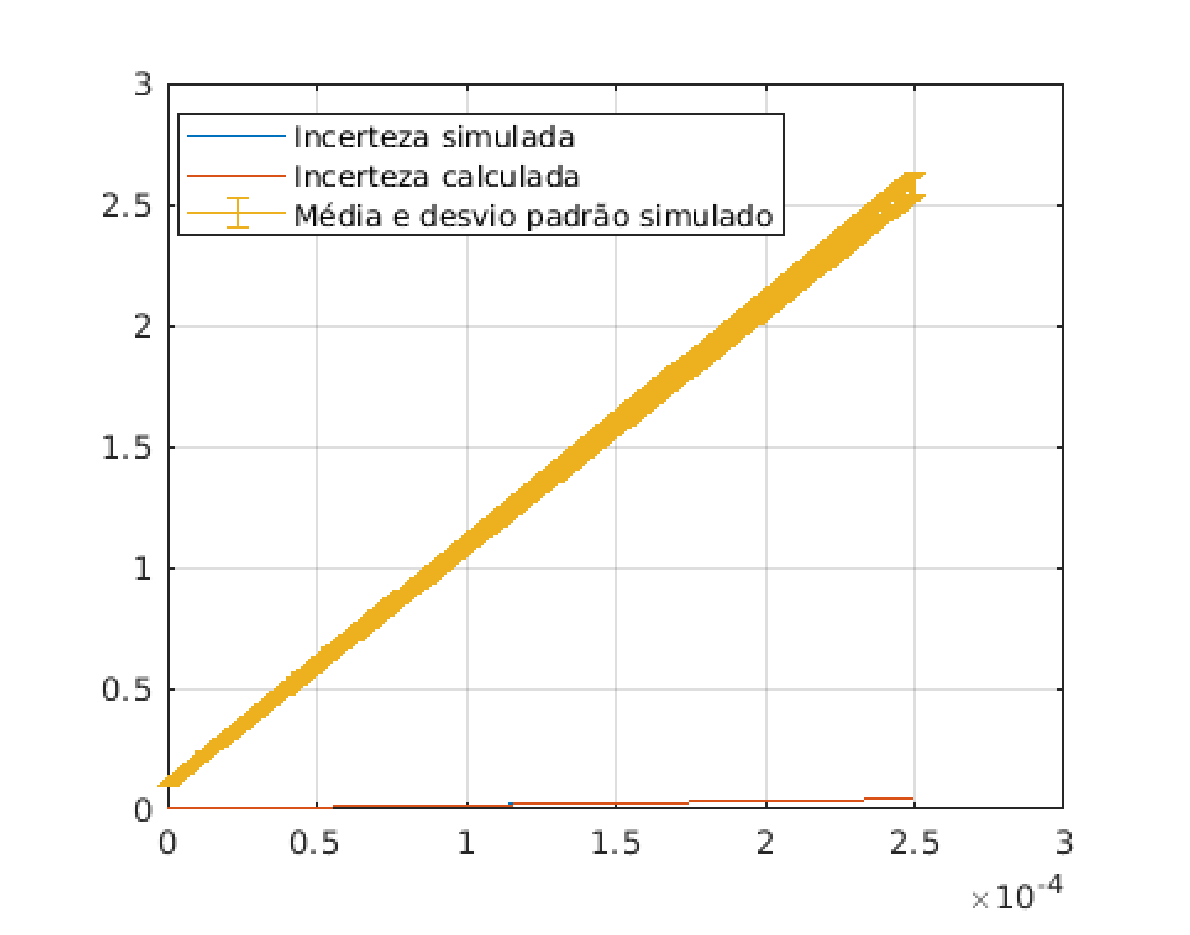
\includegraphics[keepaspectratio,totalheight=6.5in,angle=-90]{Uncertainimage5.eps}}}\end{Maple Normal}
\end{center}
}\end{Maple Normal}
\end{center}
\begin{Maple Normal}{
\begin{Maple Normal}{
}\end{Maple Normal}
}\end{Maple Normal}
\mapleinline{inert}{2d}{}{\[\displaystyle \]}
\mapleinline{inert}{2d}{}{\[\displaystyle \]}
\end{document}
